\documentclass[letterpaper]{article}
\usepackage[margin=1in]{geometry}
\usepackage[utf8]{inputenc}
\usepackage{textcomp}
\usepackage{amssymb}
\usepackage{natbib}
\usepackage{graphicx}
\usepackage{gensymb}
\usepackage{amsthm, amsmath, mathtools}
\usepackage[dvipsnames]{xcolor}
\usepackage{enumerate}
\usepackage{mdframed}
\usepackage[most]{tcolorbox}
\usepackage{csquotes}
% https://tex.stackexchange.com/questions/13506/how-to-continue-the-framed-text-box-on-multiple-pages

\tcbuselibrary{theorems}

\newcommand{\R}{\mathbb{R}}
\newcommand{\Z}{\mathbb{Z}}
\newcommand{\N}{\mathbb{N}}
\newcommand{\Q}{\mathbb{Q}}
\newcommand{\C}{\mathbb{C}}
\newcommand{\code}[1]{\texttt{#1}}
\newcommand{\mdiamond}{$\diamondsuit$}
\newcommand{\PowerSet}{\mathcal{P}}
\newcommand{\Mod}[1]{\ (\mathrm{mod}\ #1)}
\DeclareMathOperator{\lcm}{lcm}

%\newtheorem*{theorem}{Theorem}
%\newtheorem*{definition}{Definition}
%\newtheorem*{corollary}{Corollary}
%\newtheorem*{lemma}{Lemma}
\newtheorem*{proposition}{Proposition}


\newtcbtheorem[number within=section]{theorem}{Theorem}
{colback=green!5,colframe=green!35!black,fonttitle=\bfseries}{th}

\newtcbtheorem[number within=section]{definition}{Definition}
{colback=blue!5,colframe=blue!35!black,fonttitle=\bfseries}{def}

\newtcbtheorem[number within=section]{corollary}{Corollary}
{colback=yellow!5,colframe=yellow!35!black,fonttitle=\bfseries}{cor}

\newtcbtheorem[number within=section]{lemma}{Lemma}
{colback=red!5,colframe=red!35!black,fonttitle=\bfseries}{lem}

\newtcbtheorem[number within=section]{example}{Example}
{colback=white!5,colframe=white!35!black,fonttitle=\bfseries}{def}

\newtcbtheorem[number within=section]{note}{Important Note}{
        enhanced,
        sharp corners,
        attach boxed title to top left={
            xshift=-1mm,
            yshift=-5mm,
            yshifttext=-1mm
        },
        top=1.5em,
        colback=white,
        colframe=black,
        fonttitle=\bfseries,
        boxed title style={
            sharp corners,
            size=small,
            colback=red!75!black,
            colframe=red!75!black,
        } 
    }{impnote}
\usepackage[utf8]{inputenc}
\usepackage[english]{babel}
\usepackage{fancyhdr}
\usepackage[hidelinks]{hyperref}

\pagestyle{fancy}
\fancyhf{}
\rhead{CSE 101}
\chead{Friday, February 25, 2022}
\lhead{Lecture 20}
\rfoot{\thepage}

\setlength{\parindent}{0pt}

\begin{document}

\section{Dynamic Programming}
We continue our discussion on dynamic programming. 

\subsection{Problem: Chain Matrix Multiplication}
How long does it take to multiply matrices? Suppose $A$ is an $n \times m$ matrix and $B$ is a $m \times k$ matrix. Then, for each entry of $C$ (which is a $n \times k$ matrix), of which there are $nk$ entries, we need to sum $m$ terms. Therefore, the runtime\footnote{We'll ignore Strassen's algorithm for the time being.} is just 
\[\BigO(nmk)\]
Suppose, now, we want to multiply three matrices $ABC$. We can multiply it two different ways since matrix multiplication is associative. That is, we can do it either way: 
\[A(BC) \qquad (AB)C\]
How long does it take to multiply each? Suppose $A$ is a $2 \times 3$ matrix, $B$ is a $3 \times 3$ matrix, and $C$ is a $3 \times 1$ matrix. 
\begin{itemize}
    \item If we did $A(BC)$, then multiplying $BC$ would take $3 \cdot 3 \cdot 1 = 9$ operations and multiplying $A(BC)$ would take $2 \cdot 3 \cdot 1 = 6$ operations. The total runtime is $9 + 6 = 15$. 
    \item If we did $(AB)C$, then multiplying $AB$ would take $2 \cdot 3 \cdot 3 = 18$ operations and multiplying $(AB)C$ would take $2 \cdot 3 \cdot 1 = 6$ operations. The total runtime is $18 + 6 = 24$. 
\end{itemize}
The point is, from this simple example, if the matrices are complicated (not square), the order that you multiply the matrices may matter a lot. 

\bigskip 

\textbf{Problem Statement:} Find the order to multiply the matrices $A_1, A_2, \dots, A_m$ that requires the fewest total operations. In particular, assume $A_1$ is an $n_0 \times n_1$ matrix, $A_2$ is an $n_1 \times n_2$ matrix, and generally $A_k$ is an $n_{k - 1} \times n_k$ matrix. 

\subsubsection{Recursion}
In order to find some sort of a recursion so we can make a dynamic programming algorithm, we can again consider the last step. For some value of $k$, the last step is: 
\[(\underbrace{A_1 A_2 \dots A_k}_{M_1}) (\underbrace{A_{k + 1} A_{k + 2} \dots A_m}_{M_2})\]
That is, we've already computed the product of $M_1$ and $M_2$, so the last step is to multiply $M_1$ and $M_2$. So, if we want to compute the big product of matrices, what's the best runtime? The number of steps is as follows: 
\begin{itemize}
    \item We first need to compute the first half; that is, $\code{CMM}(A_1, A_2, \dots, A_k)$. 
    \item We next need to compute the second half; that is, $\code{CMM}(A_{k + 1}, A_{k + 2}, \dots, A_m)$. 
    \item Finally, we need to do the final multiplication ($M_1 M_2$), which takes $n_0 n_k n_m$ operations. 
\end{itemize}
Therefore, the recursion $\code{CMM}(A_1, A_2, \dots, A_m)$ is given by 
\[\min_{k}\left(\code{CMM}(A_1, \dots, A_k) + \code{CMM}(A_{k + 1}, \dots, A_m) + n_0 n_k n_m\right)\]
Where we need to consider all possible chain matrix multiplication orders (so we need to take the minimum of all possible values of $k$). 

\subsubsection{Subproblems}
What subproblems do we need to solve? 
\begin{itemize}
    \item Remember, we cannot afford to solve all possible chain matrix multiplication problems. So, in other words, while we \emph{do} have a recursion, if we were to try every possible $k$, that would simply take too much time on its own. 
    \item We know that $\code{CMM}(A_1, \dots, A_k)$ requires $\code{CMM}(A_1, \dots, A_k)$ and $\code{CMM}(A_{k + 1}, \dots, A_m)$ for various values of $k$.
    \item Suppose we wanted to compute $\code{CMM}(A_1, \dots, A_k)$. We might need to break this down into pieces; some of those pieces will be $\code{CMM}(A_1, \dots, A_{k'})$ ($k' < k$) and some of the pieces will be $\code{CMM}(A_{k'}, \dots, A_k)$; these are all new subproblems to deal with. When we break \emph{these} down, we don't really get anything new; that is, if we tried to run $\code{CMM}(A_i, A_{i + 1}, \dots, A_{j})$ and break these into two halves, we still have consecutive intervals of these matrices. 
    \item So, the general recursive subproblem that we need to solve is of this form
    \[C(i, j) = \code{CMM}(A_i, A_{i + 1}, \dots, A_{j})\]
    for $1 \leq i \leq j \leq m$; so there are fewer than $m^2$ total subproblems. Essentially, all we're doing is We're taking some consecutive collection of indices and we want to compute the chain matrix multiplication of that. 
\end{itemize}

\subsubsection{Full Recursion}
We now talk about the components of this recursion. 
\begin{itemize}
    \item \underline{Base Case:} For the base case, $C(i, i) = 0$. All this is saying is that you want to multiply the matrix $A_i$ and that's it; so, there's only one matrix. With a single matrix, we don't need to do anything.
    \item \underline{Recursive Step:} The recursive step is given by 
    \[C(i, j) = \min_{i \leq k < j} \left(C(i, k) + C(k + 1, j) + n_i n_k n_j\right)\]
    If we have $i < j$, then $C(i, j)$ should be the \emph{minimum} of all possible places we can break this product into two pieces; in other words, it's the minimum of the two recursive calls plus the final computation. 
    \item \underline{Solution Order:} We need to solve the subproblems with smaller $j - i$ first. This ensures that the recursive calls will always be in your table.   
\end{itemize}

\subsubsection{Example: Chain Matrix Multiplication}
Suppose $A$ is a $2 \times 5$ matrix, $B$ is a $5 \times 4$ matrix, $C$ is a $4 \times 3$ matrix, and $D$ is a $3 \times 5$ matrix. 

\begin{enumerate}
    \item Compute the minimum number of operations needed to evaluate $ABCD$. 

    \begin{mdframed}[]
        We can build this table $T$: 
        \begin{center}
            \begin{tabular}{|c|c|c|c|c|}
                \hline
                         & \code{A} & \code{B} & \code{C} & \code{D} \\ 
                \hline 
                \code{A} &          &          &          &          \\
                \hline  
                \code{B} &          &          &          &          \\
                \hline 
                \code{C} &          &          &          &          \\
                \hline 
                \code{D} &          &          &          &          \\
                \hline      
            \end{tabular}
        \end{center}
        Here, we're performing chained matrix multiplication, where we start at some matrix (denoted by the row) and finish at another matrix (denoted by the column). So, if we chose the row $A$ and the column $C$, this means $ABC$. Thus, $T[X, Y]$ means that we start at matrix $X$ and end at matrix $Y$. Thus, we're interested in finding the value of $T[A, D]$ since this means the number of steps needed to compute $ABCD$. 
    
        \begin{itemize}
            \item First, we note that the bottom-left diagonal calls make no sense. For example, we don't need $T[C, B]$ as this is saying the number of operations needed to compute $CB$, but we will never need a subproblem where this is the case. So: 
            \begin{center}
                \begin{tabular}{|c|c|c|c|c|}
                    \hline
                             & \code{A} & \code{B} & \code{C} & \code{D} \\ 
                    \hline 
                    \code{A} &          &          &          &          \\
                    \hline  
                    \code{B} & \code{X} &          &          &          \\
                    \hline 
                    \code{C} & \code{X} & \code{X} &          &          \\
                    \hline 
                    \code{D} & \code{X} & \code{X} & \code{X} &          \\
                    \hline      
                \end{tabular}
            \end{center}
    
            \item Next, we start with the base case. That is, $T[A, A] = T[B, B] = T[C, C] = T[D, D] = 0$. So: 
            \begin{center}
                \begin{tabular}{|c|c|c|c|c|}
                    \hline
                             & \code{A} & \code{B} & \code{C} & \code{D} \\ 
                    \hline 
                    \code{A} &    0     &          &          &          \\
                    \hline  
                    \code{B} & \code{X} &    0     &          &          \\
                    \hline 
                    \code{C} & \code{X} & \code{X} &    0     &          \\
                    \hline 
                    \code{D} & \code{X} & \code{X} & \code{X} &    0     \\
                    \hline      
                \end{tabular}
            \end{center}
    
            \item Next, we look at $T[A, B]$. Recall that $A$ is a $2 \times 5$ matrix and $B$ is a $5 \times 4$ matrix. Further, there is only \emph{one} way to break down $AB$: as itself. So it follows that $AB$ will take $2 \cdot 5 \cdot 4 = 40$ operations to compute. 
            \begin{center}
                \begin{tabular}{|c|c|c|c|c|}
                    \hline
                             & \code{A} & \code{B} & \code{C} & \code{D} \\ 
                    \hline 
                    \code{A} &    0     &    40    &          &          \\
                    \hline  
                    \code{B} & \code{X} &    0     &          &          \\
                    \hline 
                    \code{C} & \code{X} & \code{X} &    0     &          \\
                    \hline 
                    \code{D} & \code{X} & \code{X} & \code{X} &    0     \\
                    \hline      
                \end{tabular}
            \end{center}
    
            \item Next, we look at $T[B, C]$. Again, there's only one way to break this down -- as itself. So, it follows that $BC$ will take $5 \cdot 4 \cdot 3 = 60$ operations to compute. 
            \begin{center}
                \begin{tabular}{|c|c|c|c|c|}
                    \hline
                             & \code{A} & \code{B} & \code{C} & \code{D} \\ 
                    \hline 
                    \code{A} &    0     &    40    &          &          \\
                    \hline  
                    \code{B} & \code{X} &    0     &    60    &          \\
                    \hline 
                    \code{C} & \code{X} & \code{X} &    0     &          \\
                    \hline 
                    \code{D} & \code{X} & \code{X} & \code{X} &    0     \\
                    \hline      
                \end{tabular}
            \end{center}
    
            \item For the same reason as above, $T[C, D]$ will take $4 \cdot 3 \cdot 5 = 60$ operations to compute. 
            \begin{center}
                \begin{tabular}{|c|c|c|c|c|}
                    \hline
                             & \code{A} & \code{B} & \code{C} & \code{D} \\ 
                    \hline 
                    \code{A} &    0     &    40    &          &          \\
                    \hline  
                    \code{B} & \code{X} &    0     &    60    &          \\
                    \hline 
                    \code{C} & \code{X} & \code{X} &    0     &    60    \\
                    \hline 
                    \code{D} & \code{X} & \code{X} & \code{X} &    0     \\
                    \hline      
                \end{tabular}
            \end{center}
    
            \item Next, we look at $T[A, C]$. Since there are three matrices here, there are two ways to break this down. 
            \begin{itemize}
                \item $A(BC)$: Note that $BC$ will be a $5 \times 3$ matrix. Since $A$ is a $2 \times 5$ matrix, it follows that 
                \[2 \cdot 5 \cdot 3 + T[B, C] = 30 + 60 = 90\]
                \item $(AB)C$: Note that $AB$ will be a $2 \times 4$ matrix. Since $C$ is a $4 \times 3$ matrix, it follows that 
                \[T[A, B] + 2 \cdot 4 \cdot 3 = 40 + 24 = 64\]
            \end{itemize}
            Taking the minimum of the total number of ways to break this problem down, we have \textbf{64}. So: 
            \begin{center}
                \begin{tabular}{|c|c|c|c|c|}
                    \hline
                             & \code{A} & \code{B} & \code{C} & \code{D} \\ 
                    \hline 
                    \code{A} &    0     &    40    &    64    &          \\
                    \hline  
                    \code{B} & \code{X} &    0     &    60    &          \\
                    \hline 
                    \code{C} & \code{X} & \code{X} &    0     &    60    \\
                    \hline 
                    \code{D} & \code{X} & \code{X} & \code{X} &    0     \\
                    \hline      
                \end{tabular}
            \end{center}
    
            \item Next, we look at $T[B, D]$. Since there are three matrices here, there are two ways to break this down as well. 
            \begin{itemize}
                \item $B(CD)$: Note that $CD$ is a $4 \times 5$ matrix. Since $B$ is a $5 \times 4$ matrix, it follows that 
                \[5 \cdot 4 \cdot 5 + T[C, D] = 100 + 60 = 160\]
                \item $(BC)D$: Note that $BC$ is a $5 \times 3$ matrix. Since $D$ is a $3 \times 5$ matrix, it follows that 
                \[T[B, C] + 5 \cdot 3 \cdot 5 = 60 + 75 = 135\]
            \end{itemize}
            Taking the minimum of the total number of ways to break this problem down, we have \textbf{135}. So: 
            \begin{center}
                \begin{tabular}{|c|c|c|c|c|}
                    \hline
                            & \code{A} & \code{B} & \code{C} & \code{D} \\ 
                    \hline 
                    \code{A} &    0     &    40    &    64    &          \\
                    \hline  
                    \code{B} & \code{X} &    0     &    60    &    135   \\
                    \hline 
                    \code{C} & \code{X} & \code{X} &    0     &    60    \\
                    \hline 
                    \code{D} & \code{X} & \code{X} & \code{X} &    0     \\
                    \hline      
                \end{tabular}
            \end{center}
    
            \item Finally, we look at $T[A, D]$. Since there are four matrices here, there are three ways to break this down. 
            \begin{itemize}
                \item $A(BCD)$: Here, we know that $T[B, D] = 135$. Additionally, since $BCD$ is a $5 \times 5$ matrix and $A$ is a $2 \times 5$ matrix, it follows that 
                \[2 \cdot 5 \cdot 5 + 135 = 185\]
                \item $(AB)(CD)$: Here, we know that $AB$ is a $2 \times 4$ matrix and $CD$ is a $4 \times 5$ matrix. Additionally, $T[A, B] = 40$ and $T[C, D] = 60$. So, it follows that 
                \[T[A, B] + 2 \cdot 4 \cdot 5 + T[C, D] = 40 + 40 + 60 = 140\]
                \item $(ABC)D$: Here, we know that $ABC$ is a $2 \times 3$ matrix and $D$ is a $3 \times 5$ matrix. Additionally, $T[A, C] = 64$. So, it follows that 
                \[T[A, C] + 2 \cdot 3 \cdot 5 = 64 + 30 = 94\]
            \end{itemize}
            Taking the minimum of the total number of ways to break this problem down, we have \textbf{94}. So: 
            \begin{center}
                \begin{tabular}{|c|c|c|c|c|}
                    \hline
                            & \code{A} & \code{B} & \code{C} & \code{D} \\ 
                    \hline 
                    \code{A} &    0     &    40    &    64    &    94    \\
                    \hline  
                    \code{B} & \code{X} &    0     &    60    &    135   \\
                    \hline 
                    \code{C} & \code{X} & \code{X} &    0     &    60    \\
                    \hline 
                    \code{D} & \code{X} & \code{X} & \code{X} &    0     \\
                    \hline      
                \end{tabular}
            \end{center}
        \end{itemize}
        Therefore, our solution is given by $T[A, D] = \textbf{94}$. 
    \end{mdframed}

    \item What order did you have to multiply the matrices to get the lowest possible of computations? 
    \begin{mdframed}[]
        We note that the least number of computations needed to evaluate $ABCD$ is given by 94. Like with the other examples, we can backtrack to figure out the order. 
        \begin{itemize}
            \item In order to get $T[A, D] = 94$, we had to compute $(ABC)D$. So, we need to go back to $T[A, C]$, which is 64. 
            \item Looking at $T[A, C] = 64$, we see that the we had to compute $(AB)C$. So, we need to go back to $T[A, B]$, which is 40.
            \item Looking at $T[A, B]$, there's only one way to multiply $AB$. So, we're done.  
        \end{itemize}
        From this, it follows that the order in which we multiplied these matrices is 
        \[ABCD \implies (ABC)D \implies \boxed{((AB)C)D}\]
    \end{mdframed}
    \textbf{Remark:} If we have a tie somewhere, this implies that there is more than one optimal solution. So, you can return one of the optimal solutions. 
\end{enumerate}

\subsubsection{Runtime}
The runtime of this algorithm is given by: 
\begin{itemize}
    \item \underline{Number of Subproblems:} We needed to index through all possible $(i, j)$ in the range $1 \leq i \leq j \leq m$. So, the total number of subproblems is at most $m^2$.
    \item \underline{Time per Subproblem:} We need to check each $i \leq k < j$ as one of your terms for the maximum. Each check takes constant time (two table lookups and some multiplication and additions). We need to check $m$ different values of $k$.
\end{itemize}
Thus, we have 
\[\BigO(m^2 m) = \BigO(m^3)\]

\subsubsection{Dynamic Programming Setup}
Sometimes, there are many ways to create a dynamic programming algorithm for a given problem. How we set it up will have a large effect on the runtime. 


\subsection{All Pairs Shortest Paths}
\textbf{Problem Statement:} Given a directed graph $G$ with possibly negative edge weights, compute the length of the shortest path between \underline{every pair} of vertices\footnote{Bellman-Ford computes the single-source shortest paths. Namely, for some fixed vertex $s$, it computes all of the shortest path lengths $d(s, v)$ for every $v$. In \emph{this} problem, we want to compute the shortest path from every vertex to every other vertex.}.

\subsubsection{Naive Algorithm}
The easy algorithm is to run Bellman Ford with source $s$ for each vertex $s$. The runtime is given by $\BigO(|V|^2 |E|)$. 

\subsubsection{Dynamic Program}
Let $d_{k}(u, v)$ be the length of the shortest path from $u$ to $v$ that uses at most $k$ edges. 
\begin{center}
    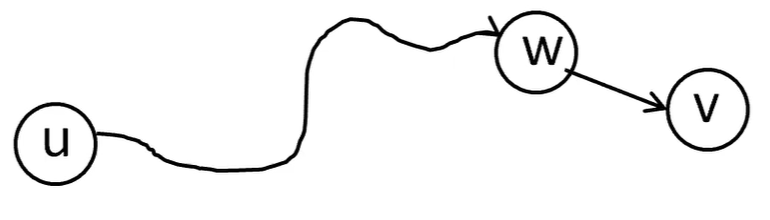
\includegraphics[scale=0.3]{../assets/sp.png}
\end{center}
So, we can consider the last edge of that path; in our case, $w$ to $v$. Then, we have the path with length $k - 1$ from $u$ to $w$ followed by the edge $w$ to $v$. So: 
\[d_{k}(u, v) = \min_{w \in V}(d_{k - 1}(u, w) + \ell(w, v))\]

\subsubsection{Matrix Multiplication Method}
We know that Bellman Ford is slow in part because we can only increase $k$ by one step at a time. This happens because we cut off only the last edge of the optimal path. However, for computation distances from every vertex to every other vertex, there's a better way to do this. What if, instead, we cut this path in the middle in the middle instead of just one edge off of the end like we do with Bellman Ford?

\subsubsection{Recursion}
Suppose we have a path $u$ to $v$ with at most $2k$ edges: 
\begin{center}
    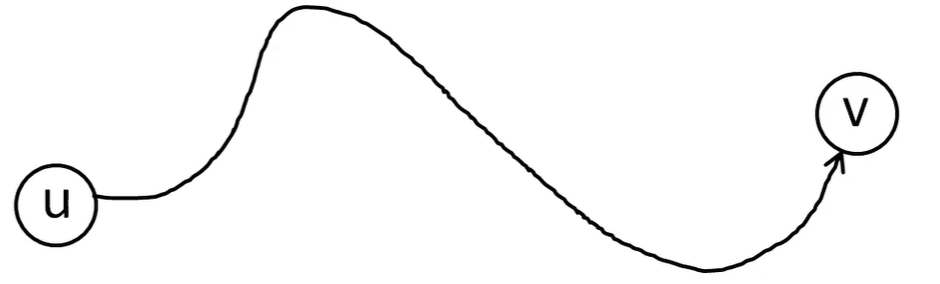
\includegraphics[scale=0.5]{../assets/sp_2.png}
\end{center}
Then, we can always pick a vertex $w$ so that there are at most $k$ edges on either side of it, like so: 
\begin{center}
    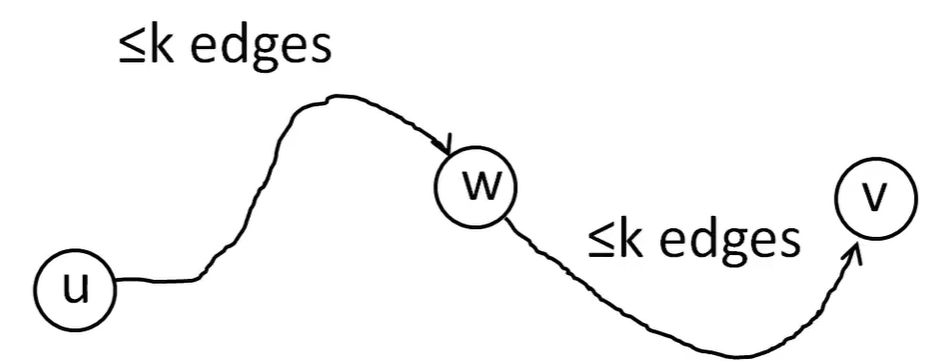
\includegraphics[scale=0.5]{../assets/sp_3.png}
\end{center}
If we picked a particular vertex $w$, then the best length we will get is 
\[d_{2k}(u, v) = \min_{w \in V} (d_{k}(u, w) + d_{k}(w, v))\]
It's not hard to see that $d_{2k}(u, v)$ is just the minimum over all vertices $w$ that go in the middle. This gives us a somewhat different recurrence relation, and a totally different dynamic program for computing all pairs shortest path. 


\subsubsection{Algorithm}
How does the algorithm work? 

\begin{itemize}
    \item \underline{Base Case:} The base case is given by the path length if we only have 1 edge. 
    \[d_{1}(u, v) = \begin{cases}
        0 & \text{if } u = v \\ 
        \ell(u, v) & \text{if } (u, v) \in E \\ 
        \infty & \text{otherwise (no edge)} 
    \end{cases}\]

    \item \underline{Recursion:} Given $d_{k}(u, v)$ for all $u, v$, we can compute $d_{2k}(u, v)$ using 
    \[d_{2k}(u, v) = \min_{w \in V} (d_{k}(u, w) + d_{k}(w, v))\]

    \item \underline{End Condition:} We can compute $d_1, d_2, d_4, d_8, d_{16}, \dots, d_m$ until $m > |V|$. 
\end{itemize}

The base case takes $\BigO(|V|^2)$ time to fill the initial table. The recursion takes $\BigO(|V|^3)$; this is because we need to consider every pair, of which there are $|V|^2$ possibilities, and then taking the minimum of all third vertices. Finally, the end condition takes $\BigO(\log(|V|))$ time. Thus, the runtime is given by 
\[\BigO(|V|^3 \log(|V|))\]


\subsubsection{Floyd-Warshall Algorithm}
We can look at this problem in a different way. 
\begin{itemize}
    \item First, we \emph{label} the vertices $v_1, v_2, \dots, v_n$, where $n$ is the total number of vertices. 
    \item Next, we define $d_{k}(u, v)$ be the length of the shortest path from $u$ to $w$ using only $v_1, v_2, \dots, v_k$ as intermediate vertices. So, we are restricting what vertices we can use to get from one vertex to the other. 
\end{itemize}
Thus, the algorithm is given by: 
\begin{itemize}
    \item \underline{Base Case:} The base case is given by the fact that you aren't allowed to use any intermediate vertices. So: 
    \[d_{0}(u, v) = \begin{cases}
        0 & \text{if } u = v \\ 
        \ell(u, v) & \text{if } (u, v) \in E \\ 
        \infty & \text{otherwise (no edge)} 
    \end{cases}\]

    \item \underline{Recursion:} Suppose we want to get from $u$ to $w$ using only vertices $v_1, \dots, v_k$. We will consider several different cases depending on whether or not the shortest path uses $v_k$.
    \begin{itemize}
        \item If the shortest path does not use $v_k$, then it only uses the intermediate vertices $v_1, v_2, \dots, v_{k - 1}$. Thus, the shortest path is given by $d_{k - 1}(u, w)$. 
        \item If the shortest path does use $v_k$, then we can break this path down like so: 
        \begin{center}
            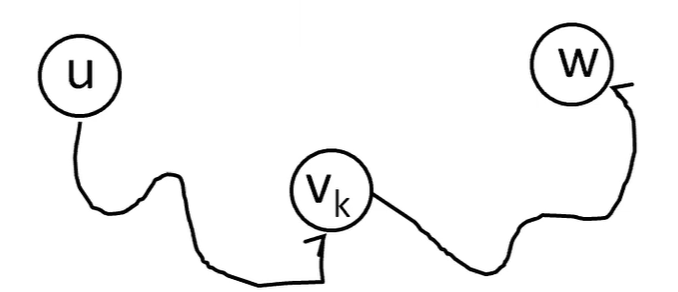
\includegraphics[scale=0.5]{../assets/sp3.png}
        \end{center}
        It has length 
        \[d_{k - 1}(u, v_k) + d_{k - 1}(v_k, w)\]
        We can start at $u$, move through some intermediate vertices to get to $v_k$, and then move through more intermediate vertices to get to $w$. In either cases, the intermediate vertices can be $v_1$ to $v_{k - 1}$. 
    \end{itemize}
    In other words, for each $u$ and $w$, we want to compute 
    \[d_{k}(u, v) = \min(d_{k - 1}(u, w), d_{k - 1}(u, v_k) + d_{k - 1}(v_k, w))\]

    \item \underline{End Condition:} The end condition is given by 
    \[d(u, w) = d_{n}(u, w)\]
    where $n = |V|$. 
\end{itemize}
The runtime is given by 
\begin{itemize}
    \item The base case takes $\BigO(|V|^2)$ time to fill up the table. 
    \item The recursion takes $\BigO(|V|^2)$ time because there are $|V|^2$ pairs to consider.
    \item The end condition takes $\BigO(|V|)$ time. 
\end{itemize}
The final runtime is then 
\[\BigO(|V|^3)\]

\subsubsection{Best Known Algorithm}
The best known algorithm doesn't actually use dynamic programming. 
\begin{enumerate}
    \item Run Bellman-Ford \emph{once} to compute $d(v)$. 
    \item Then, we reweigh the edges. We replace the length $\ell$ with $\ell'$; $\ell'$ is given by (for every edge from $u$ to $w$)
    \[\ell'(u, w) = \ell(u, w) = d(u) - d(w) \geq 0\]
    There are two things to note: 
    \begin{itemize}
        \item $\ell'(u, w)$ will always be non-negative because $d(w) \leq d(u) + \ell(u, w)$. 
        \item Computing the shortest path with $\ell'(u, w)$ is equivalent to computing the shortest path with $\ell(u, w)$. 
    \end{itemize}
    
    \item Run Dijkstra's algorithm from every source. 
\end{enumerate}
The final runtime is given by 
\[\BigO(|V||E| + |V|^2 \log(|V|))\]


\end{document}